
%----------------------------------------------------------------------------------------
%	example
%----------------------------------------------------------------------------------------
\newcommand*{\example}{\begingroup
\section{Anwendungsbeispiel}\label{sec:example}
{\noindent Die Gewonnenen Kenntnisse sollen nun in einem typischen Anwendungsszenario betrachtet werden. Eine Eingangstür erhält ein Schloss welches sich mit einem RFID Transponder entriegeln lässt. Die Spule \(L_2\) des Transponders hat einen Radius von \(r_2 = 1cm\) und \(N_2 = 100\) Windungen. Die Spule \(L_1\) des Lesegerätes ist im Schloss verbaut, hat einen Radius \(r_1 = 2cm\) und \(N_2 = 150\) Windungen. Es soll gewährleistet sein dass der Transponder in einem Abstand von \(x \leq 5cm\) ausreichend mit Energie versorgt wird. Die Betriebsspannung der Spule \(L_1\) beträgt \(U_1 = 6V\) mit einer Frequenz \(f = 125KHz\). Außerdem sei der Innenwiderstand des Lesegerätes \(R_1 = 400\Omega\). Die induzierte Spannung \(U_{ind}\) lässt sich mit dem Transpondermodell nach der Gleichung 

\begin{equation}
 U_{ind} = \omega \cdot M \cdot I
\end{equation}

\noindent berechnen\footnote{Schalk und Bienert: RFID MIFARE und kontaktlose Smartcards angewandt, S. 78}. Das Transformatorenmodell (Abbildung \ref{transformator}) interpretiert das Lesegerät und den Transponder als einen lose gekoppelten Transformator.

\begin{figure}[H]
  \centering
    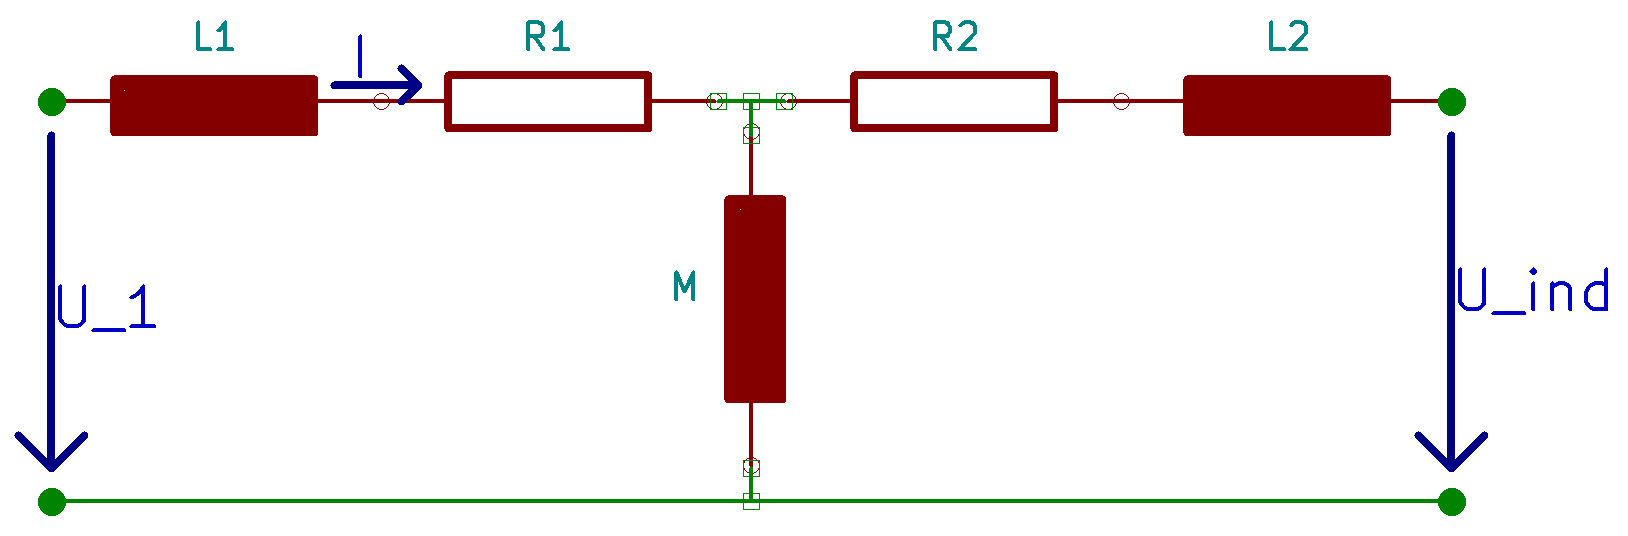
\includegraphics[width=0.9\textwidth]{Graphics/Transformator.png}
    \caption{Transformatorenmodell gekoppelter Spulen}{}
  \label{transformator}
\end{figure}

\noindent Die Kreisfrequenz \(\omega\) berechnet sich nach 

\begin{equation}
 \omega = 2\pi \cdot f
\end{equation}

\noindent Für die Gegeninduktivität \textbf{M} wird die Gleichung \eqref{eq:mutualInductance}, also 

\begin{equation}
  M = \frac{\mu \cdot \pi \cdot N_1 \cdot N_2 \cdot {r_1}^2 \cdot {r_2}^2}{2 \cdot \sqrt{(r^2 + x^2)^3}}
\end{equation}

\noindent eingesetzt, und der Strom \textbf{I} berechnet sich nach

\begin{equation}
 I = \frac{U_1}{R_1}
\end{equation}

\noindent In einem Abstand von \(x = 5cm\) induziert die Spule \(L_2\) des Transponders somit eine Spannung von 

\begin{equation}
 U_{ind} = \frac{\pi \cdot f \cdot N_1 \cdot N_2 \cdot {r_1}^2 \cdot {r_2}^2}{\sqrt{(r^2 + x^2)^3}} = 0,089V
\end{equation}

\noindent Das IC im Transponder (Abbildung \ref{transponder}) sei für eine gleichgerichtete Spannung von \(U_{IC} \approx 1V\) ausgelegt. Inklusive des Spannungsverlust an der Gleichrichtungsdiode wird also eine Spannung \(U_2 \approx 1,7V\) benötigt. Um diese zu erreichen muss der Resonanzkreis eine Güte von \(Q \approx 20\) aufweisen. Die Bedingungen zur Dimensionierung von der Spule \(L_{res}\) und dem Kondensator \(C_{res}\) des Resonanzkreises sind somit

\begin{equation}
 \omega L_{res} - \frac{1}{\omega C_{res}} = 0
 \label{eq:resonance}
\end{equation}

\noindent um die Blindwiderstände auszukompensieren und 

\begin{equation}
 Q = 20 = \frac{\omega L_{res}}{R_{res}}
\end{equation}

\noindent für die geforderte Güte. Sei angenommen, dass der reelle Widerstand \(R_{res} = 100\Omega\) ist, dann errechnet sich für die Spule \(L_{res} = 2,54mH\). Die Gleichung \eqref{eq:resonance} nach \(C_{res}\) umgestellt und das Ergebnis für \(L_{res}\) eingesetzt, ergibt eine Kapazität von \(C_{res} = 638,24pF\).

\begin{figure}[H]
  \centering
    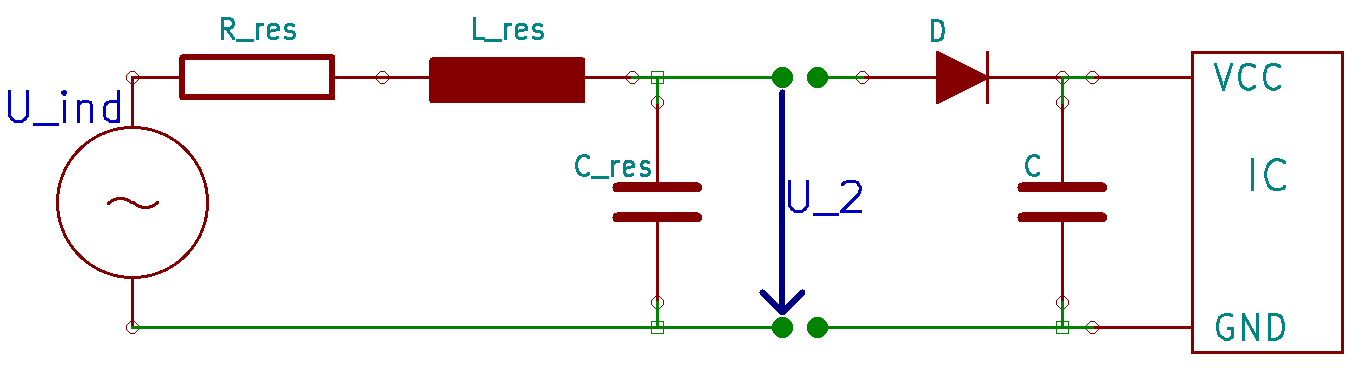
\includegraphics[width=0.9\textwidth]{Graphics/Transponder.png}
    \caption{Vereinfachte Schaltung eines Transponders}{}
  \label{transponder}
\end{figure}

}
\endgroup}
%----------------------------------------------------------------------------------------
